%%%%%%%%%%%%%%%%%%%%%%%%%%%%%%%%%%%%%%%%%%%%%%%%%%%%%%%%%%%%%%%%%%%%%%%%%
%           Capítulo 2: MARCO TEÓRICO - REVISIÓN DE LITERATURA
%%%%%%%%%%%%%%%%%%%%%%%%%%%%%%%%%%%%%%%%%%%%%%%%%%%%%%%%%%%%%%%%%%%%%%%%%
\chapter{Sistemas Hamiltonianos de dos dimensiones}
Para llegar al análisis de los sistemas de nuestro interés mediante el método de parametrización es fundamental conocer algunos conceptos sobre la dinámica así como del análisis numérico del mismo. En este capítulo se hace una breve descripción de los teoremas y definiciones que nos ayudarán a entender el método. Las siguientes secciones no son la manera más formal de introducir al lector a cada uno de los temas expuestos. Sin embargo proporcionan una visión puntual de lo indispensable. 

\section{Sistemas dinámicos}
Cuando uno habla sobre sistemas dinámicos lo que le viene a la mente es alguna relación que describe el comportamiento temporal de un sistema físico. Ya sea el movimiento de péndulos o de cargas, nos interesa saber más acerca de las características de su comportamiento. 
En el estudio de los mismos se hace una clasificación en términos de sus propiedades vistas en el espacio fase o por la forma del sistema. Hay sistemas dinámicos discretos y sistemas dinámicos continuos, en el primero el tiempo varía discretamente mientras que en el segundo varía de manera contínua. \\

 Dentro de estas características de clasificación también puede ser que el sistema sea de tipo determinista o estocástico. La diferencia entre ambos es que para el determinista dado un punto en el espacio fase existe uno y sólo un punto subsecuente bien definido, mientras que en el estocástico para un estado puede haber varios estados subsecuentes posibles.
En algunos casos los sistemas resultan ser simples, por ejemplo si su movimiento es regular. En otros sistemas, dos condiciones iniciales cercanas se alejan exponencialmente con el tiempo. En este trabajo nos enfocaremos en los  sistemas deterministas discretos.\\

Para formalizar usaremos la siguiente definición de sistema dinámico.  \\
\begin{defini}[\textsc{\textit{Sistema dinámico}}\cite{gerald}]
\textit{Un sistema dinámico es un semigrupo $G$ actuando en un espacio $M$, definido por una relación de la forma}
\begin{equation}
T : G \times M \rightarrow M; \quad
T_{g}\circ T_{h}=T_{g\circ h} . \label{def sistema dinamico}
\end{equation}
\end{defini}

Un ejemplo típico de un sistema dinámico continuo es el flujo de una ecuación diferencial autónoma, mientras que de uno discreto es por ejemplo el mapeo de un intervalo cerrado en $\mathbb{R}$ en sí mismo, o simplemente una función iterada. En el primer caso
\begin{equation}
\dot{x} =  f(x); \quad  
x(0)=x_{0} , \label{ec dif}
\end{equation}
suponiendo que $f \in C^{k}(M,\mathbb{R}^{n})$ con $k \geq 1$ y donde $M$ es un subconjunto abierto de $\mathbb{R}^{n}$. Las soluciones de este tipo de sistemas son curvas contenidas en $\mathbb{R}^{n}$ a las que llamamos trayectorias y denotamos por $\phi$.\\
En el segundo caso  
\begin{eqnarray}
\pmb x_{n+1}= \mathbf{f}(\pmb x_{n}) \quad \pmb x\in \mathbb{R}^{n}. \label{sistema discreto}
\end{eqnarray}
Para la ecuación \eqref{sistema discreto} dada una condición inicial $\pmb x_{0}$ podemos obtener el estado siguiente evaluando el lado derecho con tal punto. De manera sucesiva se puede obtener el estado $\pmb x_{n+1}$ del estado $\pmb x_{n}$. La aplicación consecutiva de la función proporciona la trayectoria u órbita del punto inicial. Podemos decir que el mapeo es un isomorfismo entre la condición inicial y los puntos de la trayectoria,
\begin{eqnarray*}
\pmb x_{k}=\mathbf{f}\circ\mathbf{f}\circ \mathbf{f} \circ \mathbf{f} ... \circ \mathbf{f} (\pmb x_{0})\quad (k \quad \textrm{veces})
\end{eqnarray*}
o
\begin{eqnarray*}
\pmb x_{k} = \mathbf{f}^{k}(\pmb x_{0}).
\end{eqnarray*}
Al conjunto $\lbrace \pmb x_{0},\pmb x_{1},...,\pmb x_{n} \rbrace$ se le llama la órbita de $\pmb x_{0}$.  En este tipo de sistemas es posible que exista un $\pmb x_{*}$ tal que $\mathbf{f}^{p}(\pmb x_{*})=\pmb x_{*}$ con $p \in \mathbb{Z}$. Es decir después de un número finito de aplicaciones se vuelve al mismo punto ($\pmb x_{*}$) al cual le llamamos un punto de periodo $p$. También es entonces posible  que exista un punto de periodo uno $\pmb x_{*}=\mathbf{f}(\pmb x_{*})$ al cual llamamos punto fijo. Los puntos fijos serán otra forma de clasificar a los sistemas dinámicos, para ello separamos las órbitas en términos de los periodos:

\begin{itemize}
\item  Órbitas fijas (asociadas a puntos con periodo uno).
\item Órbitas periódicas regulares (asociadas a puntos con periodo mayor a uno).
\item Órbitas no cerradas (asociadas a puntos no periódicos).
\end{itemize}
Nos enfocaremos sobre todo en los puntos fijos, sin embargo es posible también analizar aquellos puntos de periodo mayor a uno.
\section{Mapeos}
Como mencionamos en la introducción existen diferentes características de los sistemas dinámicos, la forma en la que depende un estado del estado anterior es una de ellas. Esa dependencia está determinada por $\mathbf{f}$ en la ecuación \eqref{sistema discreto}; gráficamente se describe en el espacio fase, que es el espacio de todos los posibles valores de $\pmb x$. En el mismo espacio la órbita de cualquier punto se ve como una trayectoria que representa la evolución de un punto $\pmb x$ bajo el mapeo hacia adelante y hacia atrás. \\

Las funciones que aparecen en el mapeo pueden contener términos con potencia mayor a uno, productos entre las variables o peor aún funciones mucho más difíciles de manejar, lo que hace que la suma de soluciones no sea solución, esa característica se llama no linealidad. Una de las primeras cosas a analizar serían los puntos fijos del sistema, los cuales deberán encontrarse algebráicamente o numéricamente dependiendo de la dificultad del mapeo, al rededor de los cuales pueden presentarse diversos comportamientos de las trayectorias.\\

Si tenemos un puno fijo $\mathbf{x}_{*}$ asociado al mapeo entonces la ecuación
\begin{eqnarray}
\mathbf{x}_{n+1} =\mathbf{A}\mathbf{x}_{n},
\end{eqnarray}
representa el sistema linearizado alrededor del punto, donde $\mathbf{A}=D\mathbf{f}(\mathbf{x}_{*})$. Es decir el mapeo puede ser representado como una matriz de coeficientes constantes, además si el sistema dinámico es invertible se puede conocer el punto anterior $\mathbf{x}_{n-1}$ a un cierto $\mathbf{x}_{n}$ usando la matriz inversa de $\mathbf{A}$ que representa la linearización del mapeo inverso $\mathbf{f}^{-1}$. Es decir las características de tal matriz nos dirán el comportamiento del sistema. \\

Dado que los sistemas tratados en este trabajo son de dos dimensiones entonces analizaremos sólo este caso. Los valores propios $\lambda_{1}, \lambda_{2}$, soluciones del polinomio característico de grado dos, son en general valores complejos clasificados como sigue.
\begin{itemize}
\item $\vert \lambda_{i}\vert<1$
\item $\vert \lambda_{i}\vert>1$
\item $\vert \lambda_{i}\vert=1$
\end{itemize}
En cada uno de los casos anteriores tenemos un vector propio $\mathbf{x}_{p1}$ asociado, tal que 
\begin{eqnarray}
\mathbf{A}\mathbf{x}_{p1}=\lambda_{1}\mathbf{x}_{p1}.
\end{eqnarray}
Los vectores serán linealmente independientes si $\lambda_{1},\lambda_{2}$ son diferentes. Si además consideramos que los valores propios son reales, según \cite{Friedberg} existe una matriz $\mathbf{U}$ tal que 
\begin{eqnarray}
\mathbf{U}^{-1}\mathbf{A}\mathbf{U} = \begin{pmatrix}
\lambda_{1} & 0\\
0 & \lambda_{2}\\
\end{pmatrix}.
\end{eqnarray}
A partir de esto es fácil ver que $\mathbf{U}$ tiene como columnas los vectores propios. Consecuentemente un mapeo lineal de dimensión dos es linealmente conjugado con un mapeo el cual tiene una matriz de representación diagonal. Este tipo de matrices son llamadas formas normales y
permiten representar el sistema en su forma más simple mediante la diagonalización del mismo \citep{arnold}.\\

Cuando los valores propios de $\mathbf{A}$ son en valor absoluto igual a uno entonces decimos que el punto fijo tiene un comportamiento elíptico. Si es el caso que un valor propio tiene valor absoluto mayor a uno y otro menor a uno entonces el punto fijo asociado es un punto fijo hiperbólico. El resultado de estas características visto en el espacio fase es un comportamiento muy particular que se muestra en la figura \ref{hiperbolic}. \\

\begin{figure}[h!]
\centering
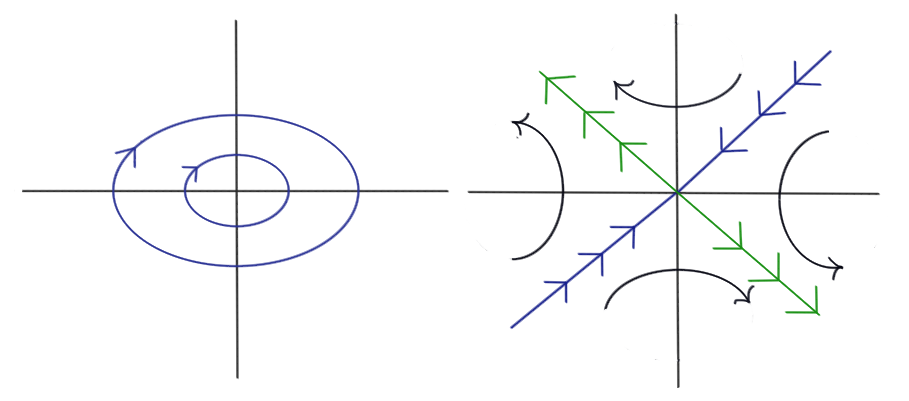
\includegraphics[scale=0.3]{hyperbolic} 
\caption{Punto fijo elíptico(izquierda) e hiperbólico(derecha) en el espacio fase.}
\label{hiperbolic}
\end{figure}


%Retomando además que si los valores propios eran ortogonales entonces podemos escribir los subespacios generados por los vectores propios.
%\begin{eqnarray*}
%E^{s}=\lbrace (x,y) : (x,y)=\beta \pmb v_{1} \quad \beta\in \mathbb{R}\rbrace
%\end{eqnarray*}
%\begin{eqnarray*}
%E^{u}=\lbrace (x,y) : (x,y)=\alpha \pmb v_{2}\quad \alpha\in \mathbb{R}\rbrace
%\end{eqnarray*}

En el caso hiperbólico tenemos dos comportamientos que nos interesan, marcados con las líneas azul y verde de la figura \ref{hiperbolic}, tales corresponden a los eigenespacios asociados a los vectores propios de $\mathbf{A}$. Existe un teorema importante de Hartman-Grobman que nos asegura que hay una vecindad del punto fijo hiperbólico tal que el mapeo es topológicamente conjugado a su linearización \cite{Meiss,Meyer,Juergen}. Dicho de otra manera, hay vecindades $U$ de $\mathbf{x}_{*}$, $V$ de $0 \in \mathbf{R}^{2}$ y un homeomorfismo $h:U\rightarrow V$ tal que $h$ mapea trayectorias de $\mathbf{f}$ en trayectorias del sistema lineal. De esta manera justificamos el porque se trabaja con un sistema lineal.



\section{Conjuntos invariantes}
Alrededor de un punto fijo existen ciertos conjuntos que nos dirán algunas características del sistema; estos conjuntos tienen que ver directamente con lo que se observa en la figura \ref{hiperbolic}. Para entender su comportamiento necesitamos definir qué es un conjunto invariante.

\begin{defini}[\textit{\textsc{Conjunto invariante}}\cite{Ott}]
\textit{Un conjunto invariante es un subconjunto $\mathbf{I} \subset \mathbf{E}$ del espacio fase tal que para cualquier $\mathbf{x}_{i}\in  \mathbf{I}$  y $ n\in\mathbb{N}$ \\
\begin{center}
$\mathbf{f}^{n}(\mathbf{x}_{i}) \in \mathbf{I}$.
\end{center}
}
\end{defini}
Es decir que cualquier elemento tomado en el conjunto se queda en el conjunto bajo la aplicación del mapeo. \\
Estudiaremos los conjuntos invariantes asociados a puntos fijos hiperbólicos. Si $\mathbf{x}_{*}$ es un punto fijo hiperbólico entonces definimos las variedades estable e inestable como
\begin{eqnarray}
W^{s}=\lbrace \mathbf{x} : \mathbf{f}^{n}(\mathbf{x})\rightarrow \mathbf{x}_{*} \quad cuando \quad n\rightarrow \infty \rbrace
\label{variedad estable}
\end{eqnarray}

\begin{eqnarray}
W^{u}=\lbrace \mathbf{x} : \mathbf{f}^{n}(\mathbf{x})\rightarrow \mathbf{x}_{*} \quad cuando \quad n\rightarrow -\infty \rbrace.
\label{variedad inestable}
\end{eqnarray}


Localmente las variedades resultan ser tangentes a los subespacios generados por los vectores propios

\begin{eqnarray*}
E^{s}=\lbrace (x,y) : (x,y)=\beta \pmb v_{1} \quad \beta\in \mathbb{R}\rbrace,
\end{eqnarray*}
\begin{eqnarray*}
E^{u}=\lbrace (x,y) : (x,y)=\alpha \pmb v_{2}\quad \alpha\in \mathbb{R}\rbrace .
\end{eqnarray*}
Esto se resume en el siguiente teorema.


%\begin{defini}[Variedad estable e inestable para un punto fijo]
%Sea \textit{$F:\mathbb{R}^{2}\rightarrow\mathbb{R}^{2}$ un  mapeo y sea $\pmb x_{*}$ un punto fijo %del mapeo , si $C \in \mathbb{R}^{2}$ es una vecindad del punto fijo  definimos}
%\begin{eqnarray*}
%W_{loc}^{s}(\pmb x_{*})=\lbrace \epsilon \in  C : \mathbf{F}^{n}(\pmb x_{i}) \in C \quad \forall n\in \mathbb{N} \rbrace
%\end{eqnarray*}
%\label{Variedad  defini}
%\end{defini}
%la definición $4$ es análoga para la variedad inestable $W_{loc}^{u}$ , pero sólo nos da una relación local. Si queremos ir más alejados del punto fijo entonces necesitamos una variedad que sea más general.Para ello existe el teorema siguiente.
%\begin{thm}[De la variedad estable(inestable)]
%\textit{Sea $\mathbf{A}$ una matriz de $2\times 2$ con dos valores propios $\lambda_{1},\lambda_{2}$ donde uno tiene parte real positiva y otro negativa, tal que si $\epsilon $ es lo suficientemente pequeña y positiva existe $ W^{s}(\pmb x_{i})$  entonces $F^{n}(\pmb x_{i})\rightarrow x_{*}$ cuando $n\rightarrow\infty$.  Respectivamente para $W^{u}(\pmb x_{i}
%)$ tenemos que $F^{n}(\pmb x_{i})\rightarrow x_{*}$ cuando $n\rightarrow -\infty$. }
%\end{thm}






%Con esto podemos asegurarar que existen funciones lo sificientemente suaves que se extienden por la %variedad, no solo de manera local. Esto es de suma importancia en el método de parametrización que %aplicaremos,ya que la parametrización se hace por medio de polinomios que son funciones suaves y %que con lo que acabamos de mencionar no sólo se aproximan de manera local. Si escribimos el %conjunto de la definición anterior
%\begin{eqnarray}
%W^{s}(\pmb x_{i})=\lbrace \pmb x_{i} \in \mathbb{R}^{2}: \lim_{n\rightarrow\infty} \mathbf{F}^{n}%(\pmb x_{i}) =x_{*}\rbrace \label{omega s}
%\end{eqnarray}
%podemos notar que además tal conjunto consiste en todas las órbitas que se acumulan bajo la %aplicación iterada del mapeo al punto fijo. En el caso en que el mapeo se a invertible entonces %podemos relacionar 
%\begin{eqnarray*}
%W^{s}(\pmb x_{*})=\cup_{n=0}^{\infty}\mathbf{F}^{n}[W_{loc}^{s}(\pmb x_{i})]
%\end{eqnarray*}
%que nos dice que la variedad estable se obtiene de la union de todas las aplicaciones hacia atrás de la variedad local estable. Para escribir de manerá análoga la variedad inestable digamos primero que la órbita hacia atrás de $\pmb x_{k}$  es $\mathbf{F}(\pmb x_{k})=\pmb x_{k+1}$ con $k\leq -1 $ donde además
%\begin{eqnarray*}
%\lim_{k\rightarrow -\infty} \pmb F(\pmb x_{k})=x_{*}
%\end{eqnarray*}
%si el mapeo es invertible entonces la órbita hacia atrás es simplemente la aplicación iterada de la %inversa. Entonces
%\begin{eqnarray*}
%W^{u}(\pmb x_{*})=\lbrace \pmb x_{i} \in \mathbb{R}^{2}: \lim_{n\rightarrow\infty} \pmb F^{n}(\pmb %x_{i})=\pmb x_{*}\rbrace \label{omega u}
%\end{eqnarray*}

%Para relacionar esto con los sistemas de interés regresemos a la ecuación \ref{sistema discreto} %donde es evidente que el origen $[0,0]$ es un punto fijo de cualquier sistema que tenga la misma forma. Si ninguno de los dos eigenvalores $\lambda_{1,2}$ de la matriz $\mathbb{A}$ tiene módulo uno  y se tiene que ambos son de signo contrario entonces la matriz es llamada hiperbólica y $x_{*}$ un punto fijo hiperbólico. Mientras que si por ejemplo los dos valores propios de $A$ tienen solo parte imaginaria entonces el sistema es llamado elíptico. El comportamiento de ambos casos se puede ver en la figura \ref{hiperbolic}. Estos conjuntos invariantes relacionados con el punto fijo resultan ser espacios propios generalizados de la matriz $\mathbb{A}$ generados por los vectores propios. Es decir si $\pmb x_{pj}=\pmb u_{j}+i\pmb v_{j}$ proviene de una base 
%\begin{eqnarray}
%\mathbf{B}=\lbrace \pmb u_{1},\pmb v_{1},\pmb u_{2},\pmb v_{2} \rbrace
%\end{eqnarray}
%entonces hay diferentes direcciones asociadas al punto fijo de acuerdo con la base $\mathbf{B}$. Para los sistemas que trabajaremos resulta que no sólo la norma de los valores propios son menores o mayores a uno, si no que además la parte imaginaria es cero para ambos. Lo que quiere decir que la base $\mathbf{B}$ tiene dos elementos únicamente. Los elementos de la misma forman subespacios, un subespacio asociado al valor propio con norma mayor a uno y otro con norma menor a uno. 

%Tomado de MAteo wirth
%\begin{thm}
%\textit{Dado un sistema de la forma \ref{sistema discreto} donde los valores propios de $\mathbb{A}$ tengan parte real diferente de cero entonces}
%\begin{eqnarray*}
%W^{s} = E^{s} 
%\end{eqnarray*}
%\begin{eqnarray*}
%W^{u}=E^{u}
%\end{eqnarray*}
%\end{thm}
%\textit{donde $E^{s}$ es la suma directa de los eigenespacios asociados al valor propio con parte real negativa , $E^{u}$ es análogo pero con positivo. En particular}
%\begin{eqnarray*}
%\mathbb{R}^{n}= W^{s}\oplus W^{u}
%\end{eqnarray*}

%Puesto que los valores propios son reales,  y entonces también los vectores propios. Este teorema nos resume que la suma directa de los conjuntos invariantes del sistema forman al espacio de soluciones. Además de mostrarnos que los conjuntos invariantes son para este caso las variedades invariantes. En el caso de sistemas más generales tenemos el siguiente teorema, que además nos aclara a qué llamamos una variedad inestable. \\


\begin{thm}[\underline{\textit{De la variedad estable}} \cite{Mateo}]
\textit{Sea un sistema de la forma $\mathbf{x}_{n+1}=\mathbf{f}(\mathbf{x}_{n})$ con un punto fijo en el origen. Sean $E^{s}$ y $E^{u}$ los subespacios estables e inestables de la linearización del sistema,$\mathbf{f}(\mathbf{x}_{n})\rightarrow\mathbb{J}\mathbf{x}_{n}$,  donde $\mathbb{J}$ es la matriz Jacobiana en el origen . Si $\mid \mathbf{f}(\mathbf{x}_{n})-\mathbb{J}\mathbf{x}_{n}\mid =O(x^{2})$ entonces existen localmente variedades estables e inestables con las mismas dimensiones que $E^{s}$,$E^{u}$ y que son tangentes a éstos en cero respectivamente.}
\begin{eqnarray*}
W^{s}_{loc}(\mathbf{x}_{*})= \lbrace \mathbf{x}_{*} : \mathbf{f}^{k}(\mathbf{x}_{n})\rightarrow \mathbf{x}_{*} cuando\quad k \rightarrow \infty \rbrace,
\end{eqnarray*}
\begin{eqnarray*}
W^{u}_{loc}(\mathbf{x}_{*}) = \lbrace \mathbf{x}_{*} : \mathbf{f}^{k}(\mathbf{x}_{n})\rightarrow \mathbf{x}_{*} cuando\quad k \rightarrow -\infty \rbrace.
\end{eqnarray*}
\end{thm}

Es necesario mencionar que una variedad estable no puede cruzarse con otra variedad estable, lo mismo sucede con las inestables, así como con la intersección de una variedad consigo misma. Para entender esto consideremos que se tienen dos puntos fijos diferentes con sus respectivas variedades inestables asociadas. Supongamos que las variedades se cruzan en algún punto. Si esto pasa la órbita hacia atrás de cualquiera de los dos puntos empezando en la intersección debería aproximarse a ambos puntos fijos, lo cual es imposible pues son diferentes. El argumento para la intersección de las estables es similar. Lo que sí puede suceder es la intersección de una variedad estable con una inestable, asociadas al mismo punto fijo; a esto se le llama una intersección homoclínica. Si la intersección es entre variedades asociadas a diferentes puntos fijos entonces se llama heteroclínica \cite{Ott}. Resulta además que si dos variedades, estable e inestable, se cortan en un punto se cortarán una infinidad de veces más. \\


El cálculo de variedades alrededor de un punto fijo es un problema difícil de atacar analíticamente, pues su comportamiento puede ser muy complejo, por ello es necesario explotar al máximo la linearización que se hace del sistema para poder, con métodos numéricos o semianalíticos, calcular las variedades. 




\section{Sistemas Hamiltonianos}
Los sistemas Hamiltonianos son una clase particular de los sistemas dinámicos. En 1834 William R. Hamilton reformuló la ecuación de Newton ($F=ma$) para un conjunto de partículas puntuales en un campo de fuerzas. Cuando la fuerza $\mathbf{F}$ es conservativa es posible escribir a la fuerza como  el negativo del gradiente de una función potencial
\begin{eqnarray}
\mathbf{F}=-\nabla V. \label{fuerza potencial}
\end{eqnarray}
Podemos convertir la ecuación \eqref{fuerza potencial} en un sistemas de ecuaciones diferenciales
\begin{eqnarray}
\frac{dx_{i}}{dt}=v_{i},
\label{fuerza sistema dif a}
\end{eqnarray}
\begin{eqnarray}
m\frac{dv_{i}}{dt}=-\nabla_{i} V.
\label{fuerza sistema dif b}
\end{eqnarray}
Las ecuaciones \eqref{fuerza sistema dif a} y \eqref{fuerza sistema dif b} pueden obtenerse a partir de una función muy particular
\begin{eqnarray}
H(q,p)=\frac{p^{2}}{2}+V(q)\sum_{n=-\infty}^{\infty}\delta(t-nT), 
\label{ec de hamilton} 
\end{eqnarray}
llamada Hamiltoniana, donde $p$ denota el momento y $q$ la posición y sin pérdida de generalidad se tomó $m=1$. De manera general, cuando se tiene un sistema de la forma
\begin{eqnarray}
H(p,q)=\frac{p^{2}}{2}+V(q),
\label{Hamiltoniano-general}
\end{eqnarray}
las ecuaciones de movimiento son
\begin{eqnarray}
\frac{dq}{dt}=\frac{\partial H}{\partial p}
\label{1ec de mov}
\end{eqnarray}
\begin{eqnarray}
\frac{dp}{dt}=-\frac{\partial H}{\partial q}.
\label{2ec de mov}
\end{eqnarray}
De aquí obtenemos para el caso de \eqref{ec de hamilton}
\begin{eqnarray}
\frac{dq}{dt}=p\quad
\label{SistemaH1}
\end{eqnarray}
\begin{eqnarray}
\frac{dp}{dt}=-\frac{dV(q)}{dq}\sum_{n=-\infty}^{\infty}\delta(t-nT),
\label{SistemaH2}
\end{eqnarray}
sin pérdida de generalidad podemos tomar $T=1$ e integrar la ecuación \eqref{SistemaH1} en el intervalo $[t_{n}-\epsilon,t_{n+1}-\epsilon]$ con $\epsilon>0$
\begin{eqnarray}
\int_{t_{n}-\epsilon}^{t_{n+1}-\epsilon}\frac{dq}{dt}dt=\int_{t_{n}-\epsilon}^{t_{n+1}-\epsilon}pdt,
\label{integral1}
\end{eqnarray}
usando el teorema fundamental del cálculo
\begin{eqnarray}
q(t_{n+1}-\epsilon)-q(t_{n}-\epsilon)=\epsilon p(t_{n}-\epsilon)+(1-\epsilon)p(t_{n+1}-\epsilon).
\label{integral2}
\end{eqnarray}
Hacemos lo mismo para la ecuación \eqref{SistemaH2}
\begin{eqnarray}
\int_{t_{n}-\epsilon}^{t_{n+1}-\epsilon}\frac{dp}{dt}dt=\int_{t_{n}-\epsilon}^{t_{n+1}-\epsilon}-\frac{dV(q)}{dq}\sum_{n=-\infty}^{\infty}\delta(t-n),
\label{integral3}
\end{eqnarray}
resultando
\begin{eqnarray}
p(t_{n+1}-\epsilon)-p(t_{n}-\epsilon)=-\frac{dV(q)}{dq}.
\label{integral4}
\end{eqnarray}
Tomando el límite cuando $\epsilon\rightarrow 0$ en las ecuaciones \eqref{integral2},\eqref{integral4} 
\begin{eqnarray}
q(t_{n+1})=p(t_{n+1})+q(t_{n}),
\label{sistema hamilton a}
\end{eqnarray}
\begin{eqnarray}
p(t_{n+1})=p(t_{n})-\frac{dV(q(t_{n}))}{dt}.
\label{sistema hamilton b}
\end{eqnarray}


%Algo análogo existe para sistemas discretos en donde la forma de la función Hamiltoniana se divide en dos partes, la derecha y la izquierda \cite{Tomoki}
%\begin{eqnarray}
%H_{d}^{+}(q_{k},p_{k+1})=p_{k+1}\cdot q_{k+1}-L_{d}(q_{k},q_{k+1}),
%\label{hamiltoniano discreto derecho}
%\end{eqnarray}

%\begin{eqnarray}
%H_{d}^{-}(p_{k},q_{k+1})=-p_{k}\cdot q_{k}-L_{d}(q_{k},q_{k+1}),
%\label{hamiltoniano discreto izquierdo}
%\end{eqnarray}

%la función $L_{d}$ es la Lagrangiana discreta que proviene del mismo principio variacional que en el caso continuo. Al definir $D_{1}F(a_{k},b_{k})=F(a_{k+1},b_{k})$ y  $D_{2}F(a_{k},b_{k})=F(a_{k},b_{k+1})$, como aplicaciones análogas a las derivadas de manera discreta  es fácil ver que las ecuaciones de movimiento análogas a las ecuaciones \ref{ec de mov hamilton} son ahora
%\begin{eqnarray}
%q_{k+1}=D_{2}H_{d}^{+}(q_{k},p_{k+1}); \quad p_{k}=D_{1}H_{d}^{+}(q_{k},p_{k+1}),
%\label{ec de mov hamilton derechas}
%\end{eqnarray}
%que también pueden ser expresadas en términos de las ecuaciones izquierdas 
%\begin{eqnarray}
%q_{k}=-D_{1}H_{d}^{-}(p_{k},q_{k+1}); \quad p_{k+1}=-D_{2}H_{d}^{-}(p_{k},q_{k+1}).
%\label{ec de mov hamilton izquierdas}
%\end{eqnarray}
%El mapeo se define de manera implícita a partir de las ecuaciones \ref{ec de mov hamilton derechas},\ref{ec de mov hamilton izquierdas} como $\mathbf{f}_{L_{d}}:(q_{k},p_{k})\mapsto(q_{k+1},p_{k+1})$.\\

%Físicamente hablando H es la energía total del sistema, que es invariante en el tiempo, $\frac{dH}{dt}=0$. La formulación Hamiltoniana de la mecánica no está limitada a sistemas que son de la forma  ``energía cinética más energía potencial'', ya que de manera más general una Hamiltoniana es cualquier función $C^{1}$, $H:M\rightarrow \mathbb{R}$ donde en nuestro caso $M$ es una variedad 2n-dimensional con coordenadas  $z=(q,p)$. 



%Para escribir las ecuaciones de Hamilton de manera resumida
%\begin{eqnarray}
%\frac{dz}{dt}=J\nabla H \label{Hamilton-poisson}
%\end{eqnarray}

%Donde $I$ es la matriz identidad de $n\times n$ por lo que $J$ es de $2n\times 2n$ antisimétrica, %llamada matriz de Poisson. 
%\begin{eqnarray*}
%J=  \begin{pmatrix}
%0 & I\\
%-I & 0
%\end{pmatrix}
%\end{eqnarray*}
%Si por otro lado pensamos que el cambio de una función escalar $F$ que depende del tiempo se puede calcular usando la ecuacion \ref{Hamilton-poisson} mediante la regla de la cadena 
%\begin{eqnarray*}
%\frac{dF}{dt}=\frac{\partial F}{\partial t}+ \lbrace F,h\rbrace
%\end{eqnarray*}
%Aquí la expresión $\lbrace F,H \rbrace$ es llamada el paréntesis de Poisson definido como:
%\begin{eqnarray}
%\lbrace F,H \rbrace=\nabla F^{T}J\nabla H \label{Parentesis Poisson}
%\end{eqnarray}
%que nos sirve para escribir las ecuaciones de movimiento \ref{ec de mov hamilton}
%\begin{eqnarray}
%\dot{z}=\lbrace z,H\rbrace \label{ec. de movimiento 2}
%\end{eqnarray}
%Algunas de las cosas que nos interesan en este tipo de sistemas son las cantidades conservadas. La %primera de ellas que nos interesa es la energía.\\

%\begin{lem}(\emph{\textit{Conservación de energía}})
%\textit{Si $H$ es independiente del tiempo entonces la energía se conserva a lo largo de trayectorias. $H(q(t),p(t))=E$.}
%\end{lem}
%\textit{\textbf{Demostración:}}
%\begin{equation*}
%\frac{dH}{dt}=\lbrace H, H \rbrace = \nabla H^{T} J \nabla H=0  
%\end{equation*}
%ya que J es antisimétrica. $\blacksquare$ \\

%La otra cantidad que nos interesa es el volumen, Joseph Liouville mostró que los flujos Hamiltonianos preservan el volumen.

%\begin{lem}(\emph{\textit{Liouville}})
%\textit{Si $H$ es $C^{2}$ entonces su flujo preserva el volumen.}
%\end{lem}

%Una carcaterística más de los sistemas Hamiltonianos es que sus puntos criticos son equivalentemente sus puntos fijos.Lo cual se enuncia en el siguiente lema. 
%\begin{lem}(\emph{Equilibrio})
%\textit{Un punto $z^{*}$ es un punto fijo del flujo autónomo Hamiltoniano si y sólo si es un punto crítico de $H$}.
%\end{lem}

%=Consecuentemente de eso tenemos que al ser iguales sus puntos críticos y fijos entonces la estabilidad de los mismos se puede estudiar a partir de la matriz Hessiana de $H$. Lo cuál analizaremos en una sección posterior. Mientras podemos pensar que una consecuencia de este lema es que cualquier máximo o mínimo no degenerdado de $H$ es Lyapunov estable. \\
%Pero ¿cómo es que este tipo de sistemas se relacionan con los sistemas lineales que analizamos antes?. La clave está en escribir a nuestro sistema de manera linearizada mediante la matriz $\mathbb{J}$. Si escribimos \ref{ec de mov hamilton} como
%\begin{eqnarray*}
%\frac{dq_{i}}{dt}=\frac{q_{i+1}-q_{i}}{\Delta t}
%\end{eqnarray*}
%donde $q_{i}=q(t)$ y $q_{i+1}=q(t+\Delta t)$. Entonces las ecuaciones de movimiento se pueden %reescribir 
%\begin{eqnarray}
%q_{i+1}=q_{i}+\Delta t p_{i} ;\quad p_{i+1}=p_{i}-\Delta t\left( \frac{\partial V}{\partial q_{i} } \right)_{q=q_{i+1}} \label{hamilton sistema dinamico}
%\end{eqnarray}
Las ecuaciones \eqref{sistema hamilton a},\eqref{sistema hamilton b} ya está en forma de un sistema de los que estudiamos anteriormente. Para linearizar el sistema calculamos el jacobiano
\begin{eqnarray}
\mathbf{J}=\frac{\partial(q_{n+1},p_{n+1})}{\partial(q_{n},p_{n})},
\end{eqnarray}
con $q_{n+1}=q(t_{n+1})$ y análogamente para $p$. Es justo de este sistema linearizado de donde obtendremos información a partir de aplicar los teoremas y resultados de las secciones anteriores. 
%Pero antes, notemos que el determinante es uno
%\begin{eqnarray*}
%det(\mathbf{J})=1+(\Delta t)^{2}\left( \frac{\partial^{2} V}{\partial q^{2} } \right)_{q=q_{i+1}}
%\end{eqnarray*}
% ya que la segunda parcial del potencial vale cero . Por lo que es un sistema que preserva áreas.









\section{Método de parametrización}
Como ya observamos en la sección anterior encontrar las variedades asociadas a un punto fijo no es trivial. Los métodos analíticos se vuelven no sólo tediosos si no que hacen necesario que el análisis de un sistema se haga de forma particular. Y para encontrar tales variedades debemos explotar los conocimientos que tenemos sobre los sistemas. Algunas de estas características son realmente simples, por ejemplo sabemos que en un punto hiperbólico resultarán dos variedades asociadas a los valores propios de la matriz que representa el sistema linearizado. Para este trabajo nos concentraremos en los sistemas Hamiltonianos ya que estos preservan el área y son importantes en la física, sin embargo el método funciona también para sistemas no Hamiltonianos. El objetivo de esta sección es describir sobre el método de parametrización el cual fue desarrollado por X.Cabré, E. Fontich y R. de la Llave \cite{Haro}. El método fue desarrollado de manera general para conjuntos invariantes, estables e inestables, en puntos hiperbólicos, tratándose de un método semianalítico, es decir parte computacional y parte analítica.\\

Para ahondar en el método recordemos que anteriormente mencionamos que los conjuntos \eqref{variedad estable}, \eqref{variedad inestable} son conjuntos invariantes. Por otro lado también recordemos la definición de sistema dinámico que nos dice que se trata de un semigrupo actuando sobre un espacio $M$, la manera en la que se genera el sistema es con un difeomorfismo $\mathbf{f}:M \rightarrow M$. En este mismo espacio $M$ definamos una inmersión inyectiva $P:\Theta \rightarrow M$ con $\theta\subset \mathbb{R}$, lo cual nos define una subvariedad $P$ parametrizada por medio de las variables locales en $\theta \in \Theta$. La variedad invariante parametrizada por $P$  junto con $g:\Theta \rightarrow \Theta$ deben cumplir 
\begin{eqnarray}
\mathbf{f} \circ P = P \circ g,  \label{Ecua de invariancia}
\end{eqnarray}
llamada ecuación de invariancia \cite{Haro}.
Es decir $P$ y $g$ son de tal forma que hacen que el siguiente diagrama conmute
\begin{eqnarray}
\xymatrix{
\Theta\subset\mathbb{R} \ar[d]^{P} \ar[r]^{g} & \Theta\subset\mathbb{R} \ar[d]^{P} \\
M\subset\mathbb{R}^{n} \ar[r]^{\mathbf{f}} & M\subset\mathbb{R}^{n}
}\label{conmutativo}
\end{eqnarray}

En este sentido $g$ representa un subsistema de $\mathbf{f}$, en otras palabras $g$ contiene la dinámica del mapeo pero sobre $\Theta$. El objetivo del método de parametrización es encontrar $P$ y $g$ que cumplan la ecuación de invariancia \eqref{Ecua de invariancia}. Aunque no conozcamos la dinámica interna de $g$ sabemos que $P$ y $g$ son soluciones de \eqref{Ecua de invariancia}, si observamos el diagrama \eqref{conmutativo} es claro que la composición también lo es y eso nos dará una libertad para resolver la ecuación. El obstáculo, no conocer $g$, se puede pasar si se escoge una forma de parametrización que dependa del sistema; en el método de parametrización se tienen descritas dos formas: la forma gráfica y la forma normal. Usaremos el método de la forma gráfica, que es la forma más simple de parametrización. Consiste en adaptar la forma de la parametrización $P$ a la forma de las variedades, la cual está relacionada con la dirección que proporcionan los vectores propios. Para el caso de una matriz hiperbólica de $2\times 2$ sus vectores propios nos indicarán, suficientemente cerca del punto fijo, la dirección de cada variedad. \\


La forma en la que se escoge $g$, en la mayoría de las veces, es polinomial de tal manera que se adapte a la forma del mapeo. Sin embargo la elección puede ser diferente dependiendo del sistema. En este caso escogimos la dependencia más sencilla para $x,y$ \eqref{fun g} que resulta ser suficiente en el caso hiperbólico
\begin{eqnarray}
g(t) = \lambda t.
\label{fun g}
\end{eqnarray}
Con esto tendremos del lado derecho de la ecuación \eqref{Ecua de invariancia} un polinomio. \\

Supongamos ahora que tenemos ya las variedades parametrizadas, para este punto es importante tener una función que nos indique qué tan acertada es nuestra parametrización. La primera y más fácil forma de calcular el error es a partir de la ecuación \eqref{Ecua de invariancia}, mediante la resta
\begin{eqnarray}
E_{n}(t) = \parallel \mathbf{f} \circ P_{n} - P_{n} \circ g \parallel_{\infty}.  \label{Ecua de invariancia resta}
\end{eqnarray}
Este error será el asociado a la variación con respecto a la ecuación de invariancia. Dado que depende del parámetro esperamos que el error vaya creciendo conforme se evalúa en valores de $t$ más alejados del punto fijo. La otra forma de evaluar qué tan lejos podemos llegar con la parametrización es ver la convergencia de los polinomios asociados. Al tener los polinomios que parametrizan la variedad, con coeficientes $a_{n}$ y $b_{n}$ de orden $n$, podemos evaluar el cociente entre ellos
\begin{eqnarray}
\lim_{n\rightarrow\infty}\frac{a_{n}}{a_{n+1}},\label{hadamard}
\end{eqnarray} 
con $(a_{0},b_{0})=\mathbf{x}_{*}$ los coeficientes de orden cero. Lo que prácticamente estamos haciendo con este cociente es lo que se llama estudiar la convergencia según Hadamard. Si el límite anterior tiende a cero entonces la serie $a_{n}$ converge. Otra forma de evaluarlo es usando la relación de tres términos \citep{Chang}.
\begin{eqnarray}
\lim_{i\rightarrow\infty} \left[ i\left(\frac{a_{i+1}}{a_{i}}\right)-(i-1)\left(\frac{a_{i}}{a_{i-1}}\right) \right].
\label{tres terminos}
\end{eqnarray}
Aunque el método se aplica de la misma manera para los puntos fijos de mapeos de dos dimensiones, la parametrización será diferente en cada mapeo y en cada punto fijo, por lo que la convergencia de cada parametrización es distinta. 